\documentclass[preprint,12pt]{elsarticle}

\usepackage{amsmath}
\usepackage{booktabs}
\usepackage{setspace}
\usepackage{url}
\usepackage{float}
\doublespacing

\journal{Knowledge-Based Systems}

\begin{document}

\begin{frontmatter}

\title{A knowledge-based early-warning system using artificial intelligence on venture data to predict digital-transformation failure in entrepreneurial firms}

\author[aff]{Hemasri Babburu\corref{cor1}}
\ead{hemasribabburu@gmail.com}
\cortext[cor1]{Corresponding author.}
\address[aff]{Doctor of Business Administration candidate. Affiliation and postal address to be inserted before submission.}

\begin{abstract}
A warning that an entrepreneurial firm will fail a digital transformation has to name the mechanism, not only rank the firm. Public venture files record closure and funding, not that failure. This Short Communication presents KBEWS, a knowledge-based early-warning system that turns seven failure mechanisms into graded rules, combines the rules by certainty factors, and anchors the resulting score to a gradient-boosting probability. The output is a calibrated probability and the rules that fired. Across 80 independent synthetic cohorts of 500 ventures, mean AUPRC is 0.683 and the mean Brier score is 0.226. Paired Wilcoxon tests against gradient boosting give $p=7.74\times10^{-13}$ for AUPRC and $p=8.15\times10^{-15}$ for the Brier score. Against the knowledge base alone, ranking does not improve (AUPRC 0.683 versus 0.681, $p=0.385$), while calibration does (Brier score 0.226 versus 0.270, $p=7.85\times10^{-15}$). The claim is limited to this mechanism-labeled benchmark. No field failure rate is estimated.
\end{abstract}

\begin{keyword}
early warning \sep knowledge-based system \sep artificial intelligence \sep digital transformation \sep entrepreneurship \sep innovation \sep venture data
\end{keyword}

\end{frontmatter}

\section{Introduction}
Digital transformation changes how a firm creates value \cite{vial2019}. The change fails when the firm cannot build the capabilities, the business-model shift, or the external links the strategy assumes \cite{warner2019,matt2016}. For an entrepreneurial firm the cost of that miss is immediate: ambition is high and slack is thin. A useful warning therefore has two outputs. It must score the risk of failure, and it must show which mechanism is active so a person can act on the score.

Those mechanisms are already named in the management literature. A capability gap, a resource misfit, a data deficit under an artificial-intelligence ambition, an imbalance between exploration and exploitation, weak external ties, missing digital leadership, and transformation without business-model adaptation recur across the strategy and innovation evidence \cite{vial2019,warner2019,oreilly2013,matt2016}. They are not columns in a public venture file. A classifier trained on closure can rank firms that shut down. It cannot tell a founder that the current transformation is failing because data maturity is behind the AI ambition, or because exploitation has pulled away from exploration.

Knowledge rules are inspectable and brittle. Data-driven models absorb residual structure and do not say which rule fired \cite{steenwinckel2021}. Certainty factors were introduced so a rule could carry a degree of belief and so several positive rules could be combined without being treated as a full probability \cite{shortliffe1975}. KBEWS uses that combination as the knowledge score and then anchors it to a gradient-boosting probability \cite{friedman2001}. The contribution is threefold: (i)~a compact, editable rule base for digital-transformation failure; (ii)~a certainty-factor anchor that returns a probability a decision maker can threshold; and (iii)~a reproducible cohort benchmark that separates what the rules contribute from what the anchor contributes. Section~\ref{sec:results} shows that the rules carry the ranking and that the anchor's distinct contribution is calibration.

\section{Proposed KBEWS framework}
\label{sec:method}

\subsection{Venture state}
Each venture is a vector of twelve indicators on $[0,1]$: digital leadership $\ell$, digital capability $c$, financial slack $s$, data maturity $m$, transformation ambition $a$, ecosystem ties $e$, exploration $x$, exploitation $i$, AI ambition $g$, business-model adaptation $b$, firm age, and firm size. Twelve irrelevant noise indicators are observed as well. They are available to the data model and invisible to the rules. Ten percent of the twelve signal values are missing. A rule whose input is missing abstains rather than being imputed.

\subsection{Knowledge-rule layer}
Seven rules convert the indicators into firing strengths in $[0,1]$. The strengths were fixed before any cohort was scored. For a gap between a driving indicator and a lagging indicator the strength is a clipped linear excess. For a joint condition the strength is the minimum of the two excesses, so both conditions must hold before the rule contributes. Writing $\mathrm{clip}(u)=\min(1,\max(0,u))$,
\begin{equation}
\begin{aligned}
s_1 &= \mathrm{clip}((a-c-0.12)/0.50), &
s_2 &= \mathrm{clip}((a-s-0.15)/0.50), \\
s_3 &= \mathrm{clip}((g-m-0.12)/0.50), &
s_4 &= \mathrm{clip}((|x-i|-0.22)/0.45), \\
s_5 &= \mathrm{clip}\!\left(\min\!\left(\tfrac{a-0.58}{0.30},\tfrac{0.40-e}{0.30}\right)\right), \\
s_6 &= \mathrm{clip}\!\left(\min\!\left(\tfrac{a-0.55}{0.30},\tfrac{0.42-\ell}{0.32}\right)\right), \\
s_7 &= \mathrm{clip}\!\left(\min\!\left(\tfrac{a-0.58}{0.30},\tfrac{0.38-b}{0.30}\right)\right).
\end{aligned}
\label{eq:rules}
\end{equation}
The seven mechanisms are capability gap, resource misfit, data deficit, ambidexterity imbalance, ecosystem isolation, leadership void, and weak adaptation. Their certainty weights are $w=(0.78,0.70,0.76,0.58,0.52,0.64,0.48)$. Positive evidence is combined by the parallel rule of Shortliffe and Buchanan \cite{shortliffe1975},
\begin{equation}
\mathrm{CF} = 1 - \prod_{k=1}^{7}\bigl(1 - w_k \tilde{s}_k\bigr),
\label{eq:cf}
\end{equation}
where $\tilde{s}_k=0$ if rule $k$ abstains and $\tilde{s}_k=s_k$ otherwise, and each factor $w_k\tilde{s}_k$ is kept below 1. CF is a degree of belief that a failure mechanism is active. It is not yet a probability that can be thresholded.

\subsection{Certainty-factor anchor}
The data model is a histogram gradient-boosting tree of depth 3, learning rate 0.08, at most 160 iterations, minimum leaf size 20, and $\ell_2$ penalty 0.1 \cite{friedman2001}. It is fit to all twenty-four indicators, with missing values left missing. It returns a failure probability $p_d$. The anchor is a logistic regression on five quantities built from out-of-fold predictions, so the anchor does not see the test ventures while it is being fit:
\begin{equation}
\begin{aligned}
\mathrm{logit}\,p ={}& b_0 + b_1\,\mathrm{logit}\,p_d + b_2\,\mathrm{CF} + b_3\,\mathrm{CF}(1-p_d) \\
& + b_4 s_{\max} + b_5 n_{50}.
\end{aligned}
\label{eq:anchor}
\end{equation}
Here $s_{\max}$ is the strongest firing and $n_{50}$ is the number of rules with strength at least 0.50. The product $\mathrm{CF}(1-p_d)$ is available to raise the warning when the data model is silent. Whether the fitted anchor uses it that way is an empirical result, reported in Section~\ref{sec:results}, not an assumption. After the anchor is fit, the tree is refit on the full training split and Eq.~\eqref{eq:anchor} is applied to the held-out ventures.

\begin{quote}
\noindent\textbf{Algorithm 1. KBEWS warning.}\\
\textit{Input:} venture indicators; the seven rules and weights in Eq.~\eqref{eq:rules}.\\
\textit{Output:} warning probability $p$ and the fired-rule trace.
\begin{enumerate}
\item Evaluate $s_1,\ldots,s_7$. A rule with a missing input abstains.
\item Combine the fired rules into CF by Eq.~\eqref{eq:cf}.
\item On the training split, build out-of-fold boosting probabilities with three stratified folds.
\item Fit Eq.~\eqref{eq:anchor} on those out-of-fold probabilities, CF, and the rule summary.
\item Refit the boosting model on the full training split and apply the anchor to the held-out ventures.
\item Return $p$ and every rule whose strength is at least 0.50.
\end{enumerate}
\end{quote}

\noindent KBEWS differs from a data-only classifier in two structural ways. The knowledge layer is a separate symbolic score, not a set of features buried inside the tree. The anchor then makes that score numerically usable, and the fired rules remain visible after the probability is issued. Figure~\ref{fig:case} shows one held-out failure in which that separation matters.

\section{Experimental design}
\label{sec:protocol}
No public venture file observes digital-transformation failure, so the experiment uses a synthetic population whose label is defined by the mechanisms the rules approximate. Each cohort contains 500 ventures drawn with its own seed. Latent leadership, capability, slack, data maturity, ambition, ecosystem ties, exploration, and exploitation are Gaussian and then clipped to $[0,1]$. AI ambition is a noisy mixture of ambition. Adaptation, age, and size are drawn independently. The failure log-odds are a stack of threshold events: a three-way corner of high ambition, low capability, and low data maturity; ambition ahead of slack; AI ambition ahead of data maturity; an exploration--exploitation gap; ambition with weak ties; ambition without digital leadership; and a protective effect when adaptation is high. A size effect under high ambition is included and is deliberately absent from Eq.~\eqref{eq:rules}, so the data model has a residual signal the rules cannot see. Gaussian noise is added on the log-odds scale. Observed indicators equal the latents plus measurement noise, and 10\% of signal cells are deleted. The mean failure rate across cohorts is 0.484. That rate describes firms already pursuing a transformation. It is not an estimate for all new firms.

Eighty cohorts give eighty matched comparisons. On each cohort a single stratified 70/30 split is drawn. Four systems are fit on that split and scored on the same held-out ventures: logistic regression on median-imputed indicators (neither the rule layer nor the nonlinear model); gradient boosting (nonlinear model, no rules); the certainty factor alone (rules, no data model); and KBEWS (both). Because each cohort is an independent draw, the paired Wilcoxon signed-rank test is the appropriate comparison of two systems across cohorts \cite{demsar2006}. Tests are two-sided. The primary ranking metric is the area under the precision--recall curve \cite{saito2015}. The primary calibration metric is the Brier score. Recall at a false-positive rate of 0.10 is the early-warning operating point. The implementation is scikit-learn \cite{pedregosa2011}. Fixed seeds make every cohort, split, and figure regenerable from the accompanying program.

\section{Results and discussion}
\label{sec:results}

\begin{table}[H]
\caption{Mean performance over 80 independent cohorts. Lower Brier scores are better. Higher values are better for AUPRC, AUROC, and recall.}
\label{tab:means}
\centering
\begin{tabular}{@{}lcccc@{}}
\toprule
Method & AUPRC & AUROC & Brier & Recall at FPR 0.10 \\
\midrule
Logistic regression & 0.630 & 0.630 & 0.244 & 0.240 \\
Gradient boosting & 0.628 & 0.623 & 0.265 & 0.246 \\
Knowledge base & 0.681 & 0.672 & 0.270 & 0.316 \\
KBEWS & 0.683 & 0.671 & 0.226 & 0.318 \\
\bottomrule
\end{tabular}
\end{table}

Table~\ref{tab:means} is the $2\times2$ reading of the system. Removing both the rule layer and the nonlinear model leaves logistic regression, with AUPRC 0.630 and Brier score 0.244. Replacing the linear model with gradient boosting does not help: AUPRC is 0.628 and the Brier score worsens to 0.265. The label is a set of thresholds, and the twelve noise indicators give the tree something to overfit. Putting the rules in and taking the data model out raises AUPRC to 0.681 and recall at a 10\% false-positive rate from 0.246 to 0.316. That is the knowledge-layer gain. Enabling both components, which is KBEWS, leaves AUPRC essentially unchanged at 0.683 and cuts the Brier score from 0.270 to 0.226.

\begin{table}[H]
\caption{Paired Wilcoxon tests of KBEWS against each of the other three systems, using the 80 matched cohorts.}
\label{tab:tests}
\centering
\begin{tabular}{@{}llccr@{}}
\toprule
Comparison & Metric & Baseline & KBEWS & $p$-value \\
\midrule
KBEWS vs.\ gradient boosting & AUPRC & 0.628 & 0.683 & $7.74\times10^{-13}$ \\
KBEWS vs.\ gradient boosting & Brier & 0.265 & 0.226 & $8.15\times10^{-15}$ \\
KBEWS vs.\ logistic regression & AUPRC & 0.630 & 0.683 & $2.35\times10^{-12}$ \\
KBEWS vs.\ logistic regression & Brier & 0.244 & 0.226 & $2.41\times10^{-13}$ \\
KBEWS vs.\ knowledge base & AUPRC & 0.681 & 0.683 & 0.385 \\
KBEWS vs.\ knowledge base & Brier & 0.270 & 0.226 & $7.85\times10^{-15}$ \\
\bottomrule
\end{tabular}
\end{table}

Table~\ref{tab:tests} separates the two claims. Against either data-only model, both ranking and calibration favor KBEWS, and the paired $p$-values are far below 0.001. Against the knowledge base alone, the AUPRC comparison is not significant ($p=0.385$). The Brier comparison is. Recall at a false-positive rate of 0.10 tells the same story: 0.318 for KBEWS, 0.316 for the knowledge base ($p=0.855$), 0.246 for gradient boosting ($p=8.19\times10^{-9}$), and 0.240 for logistic regression ($p=3.66\times10^{-10}$). A deployment that only needs a ranking can publish the certainty factor. A deployment that needs a threshold needs the anchor, because a certainty factor of 0.60 is not a 60\% probability.

Mean anchor coefficients across the 80 cohorts are $b_0=-0.57$, $b_1=0.12$, $b_2=0.69$, $b_3=-0.12$, $b_4=0.25$, and $b_5=0.39$. The certainty factor and the count of strong rules dominate. The weight on $\mathrm{logit}\,p_d$ is small. The disagreement product $\mathrm{CF}(1-p_d)$ receives a small negative weight, so the fitted anchor does not implement a rule of the form ``raise the warning only when the data model is silent.'' It treats CF as the level of the warning and uses the data model as a weak adjustment. That is why KBEWS and the knowledge base rank ventures almost equally, while their probabilities do not.

Figure~\ref{fig:case} makes the trace concrete on one held-out failure. Data maturity is 0.125 and AI ambition is 0.622, so rule R3 (data deficit) fires at strength 0.754. Exploration is 0.480 and exploitation is 0.978, so rule R4 (ambidexterity imbalance) fires at strength 0.617. Firm age is unobserved and does not enter a rule. The gradient-boosting model assigns probability 0.042. The certainty factor is 0.809. KBEWS assigns 0.785. A threshold of 0.5 would have cleared this venture on the data model and flagged it on KBEWS. The panel is one audited case, not a performance summary.

\begin{figure}[H]
\centering
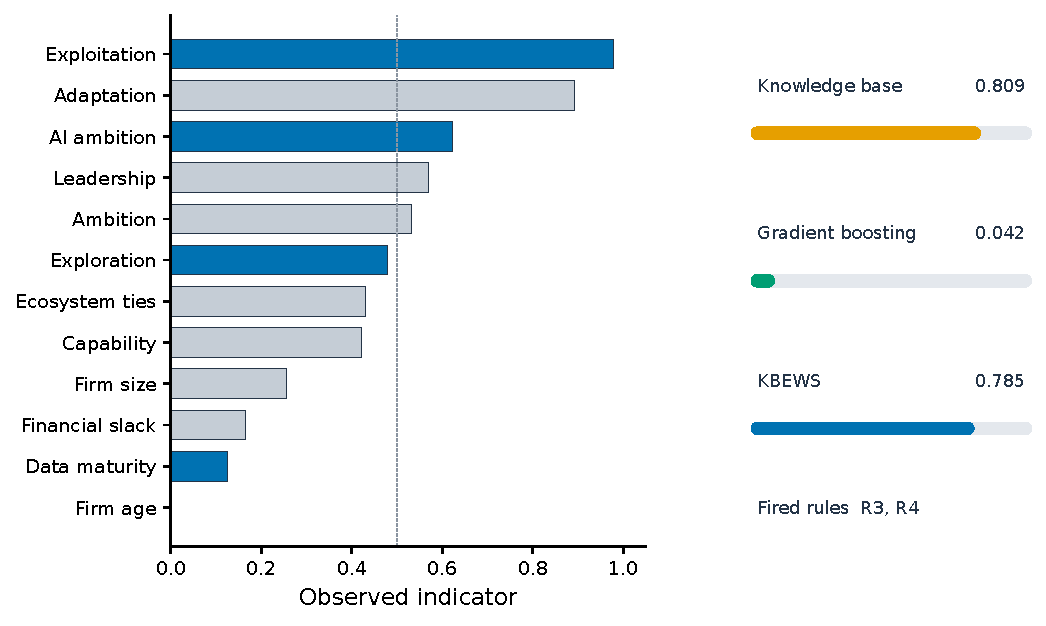
\includegraphics[width=\textwidth]{Figure_1.pdf}
\caption{One held-out failure. Blue bars are inputs of rules that fired (R3, data deficit; R4, ambidexterity imbalance). Gray bars are observed indicators that did not enter a fired rule. Firm age was missing. The right-hand strips are the knowledge score, the data-only probability, and the KBEWS probability for the same venture.}
\label{fig:case}
\end{figure}

Figure~\ref{fig:reliability} shows why the Brier result matters. Predicted probabilities from all 12{,}000 held-out venture-rows are grouped into equal-width bins, and the vertical axis is the observed failure frequency in each bin. The knowledge score lies above the diagonal through the middle of the range: a moderate certainty factor overstates the failure frequency, and the score rarely approaches zero. Gradient boosting lies below the diagonal once the predicted probability is high, so a large $p_d$ understates the failure frequency. KBEWS tracks the diagonal from about 0.4 upward. The anchor does not create a new ranking. It converts the rule score into a probability whose stated value is closer to the frequency a decision maker will actually observe.

\begin{figure}[H]
\centering
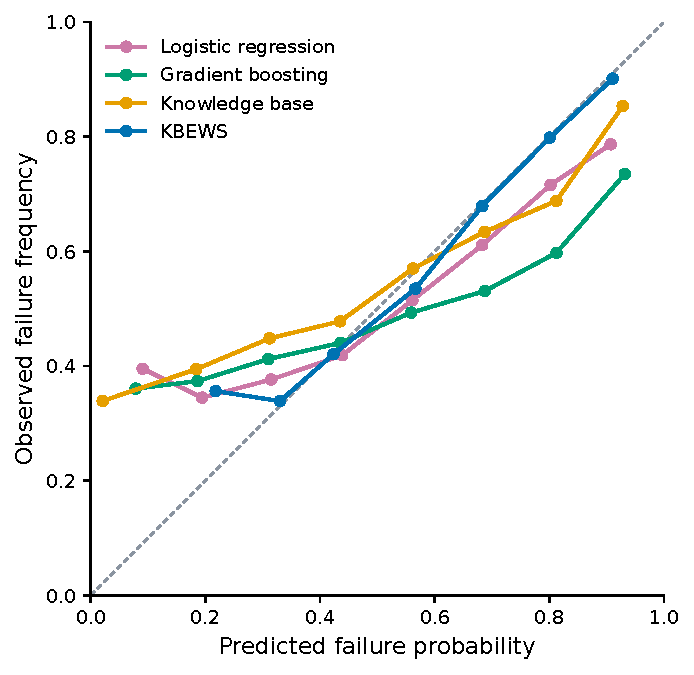
\includegraphics[width=0.86\textwidth]{Figure_2.pdf}
\caption{Reliability of the four scores on the pooled held-out rows ($n=12{,}000$). The dashed line is perfect calibration. A point is the mean predicted probability in an equal-width bin against the observed failure frequency in that bin. Bins with fewer than 40 rows are omitted.}
\label{fig:reliability}
\end{figure}

The result places KBEWS inside knowledge-based decision support rather than inside black-box prediction. The venture is flagged because named rules fired and the anchored probability crossed a threshold the user can set. Explainability comes from Eq.~\eqref{eq:rules} and Eq.~\eqref{eq:cf}, not from a post-hoc importance method applied after the tree has hidden the mechanism.

\section{Limitations}
The benchmark contains no person-level attributes, so sex and gender were neither measured nor analyzed. The stronger limit is external validity. Indicators, missingness, noise covariates, and the failure label are generated. Nothing in Table~\ref{tab:means} estimates how often real entrepreneurial firms fail at digital transformation, and the rule weights are a specification, not a record of what founders believe. The anchor also does not improve ranking over the rules; a paper that claimed an accuracy gain over the knowledge base would be claiming a result this design does not support. Replacing the generator with a file that uses the same columns and an observed failure label does not require a change to the rules or to Eq.~\eqref{eq:anchor}. Until that file exists, the numbers justify the system. They do not justify an industry claim.

\section{Conclusion}
This Short Communication presented KBEWS, a knowledge-based early-warning system for digital-transformation failure in entrepreneurial firms. Seven graded rules produce a certainty factor. A gradient-boosting model produces a data-driven probability. A logistic anchor returns one probability and leaves the fired rules visible. Across 80 independent cohorts the rules, not the data model, carry the ranking. The anchor's contribution is calibration: the Brier score falls from 0.270 to 0.226, and the reliability curve moves onto the diagonal, while AUPRC is statistically unchanged from the knowledge base alone. KBEWS is a decision-support layer. Its output is a warning a person can threshold and a mechanism a person can inspect.

{\singlespacing
\section*{CRediT authorship contribution statement}
Hemasri Babburu: Conceptualization, Methodology, Software, Validation, Formal analysis, Investigation, Data curation, Visualization, Writing -- original draft, Writing -- review and editing.

\section*{Declaration of competing interest}
The author declares that they have no known competing financial interests or personal relationships that could have appeared to influence the work reported in this paper.

\section*{Funding}
This research did not receive any specific grant from funding agencies in the public, commercial, or not-for-profit sectors.

\section*{Data availability}
The data used in this study are synthetic and reproducible. \texttt{kbews.py}, with seed 23, generates the cohorts, the paired tests, Figure~\ref{fig:case}, and Figure~\ref{fig:reliability}. No third-party microdata and no personal data were used.

\section*{Declaration of generative AI and AI-assisted technologies in the manuscript preparation process}
During the preparation of this work the author used Cursor (Grok 4.7) for language drafting and to implement the experiment code. The tables and figures were generated by that code. After using this tool, the author reviewed and edited the content as needed and takes full responsibility for the content of the published article.

\small
\begin{thebibliography}{10}

\bibitem{vial2019}
G. Vial, Understanding digital transformation: A review and a research agenda, J. Strateg. Inf. Syst. 28 (2) (2019) 118--144. \newline\url{https://doi.org/10.1016/j.jsis.2019.01.003}

\bibitem{warner2019}
K.S.R. Warner, M. W\"ager, Building dynamic capabilities for digital transformation: An ongoing process of strategic renewal, Long Range Plann. 52 (3) (2019) 326--349. \newline\url{https://doi.org/10.1016/j.lrp.2018.12.001}

\bibitem{matt2016}
C. Matt, T. Hess, A. Benlian, F. Wiesb\"ock, Options for formulating a digital transformation strategy, MIS Q. Exec. 15 (2) (2016) 123--139. \newline\url{https://aisel.aisnet.org/misqe/vol15/iss2/6/}

\bibitem{oreilly2013}
C.A. O'Reilly, M.L. Tushman, Organizational ambidexterity: Past, present, and future, Acad. Manage. Perspect. 27 (4) (2013) 324--338. \newline\url{https://doi.org/10.5465/amp.2013.0025}

\bibitem{steenwinckel2021}
B. Steenwinckel, D. De Paepe, S. Vanden Hautte, P. Heyvaert, M. Bentefrit, P. Moens, A. Dimou, B. Van Den Bossche, F. De Turck, S. Van Hoecke, F. Ongenae, FLAGS: A methodology for adaptive anomaly detection and root cause analysis on sensor data streams by fusing expert knowledge with machine learning, Future Gener. Comput. Syst. 116 (2021) 30--48. \newline\url{https://doi.org/10.1016/j.future.2020.10.015}

\bibitem{shortliffe1975}
E.H. Shortliffe, B.G. Buchanan, A model of inexact reasoning in medicine, Math. Biosci. 23 (1975) 351--379. \newline\url{https://doi.org/10.1016/0025-5564(75)90047-4}

\bibitem{friedman2001}
J.H. Friedman, Greedy function approximation: A gradient boosting machine, Ann. Stat. 29 (5) (2001) 1189--1232. \newline\url{https://doi.org/10.1214/aos/1013203451}

\bibitem{saito2015}
T. Saito, M. Rehmsmeier, The precision-recall plot is more informative than the ROC plot when evaluating binary classifiers on imbalanced datasets, PLoS One 10 (3) (2015) e0118432. \newline\url{https://doi.org/10.1371/journal.pone.0118432}

\bibitem{demsar2006}
J. Dem\v{s}ar, Statistical comparisons of classifiers over multiple data sets, J. Mach. Learn. Res. 7 (2006) 1--30.

\bibitem{pedregosa2011}
F. Pedregosa, G. Varoquaux, A. Gramfort, V. Michel, B. Thirion, O. Grisel, M. Blondel, P. Prettenhofer, R. Weiss, V. Dubourg, J. Vanderplas, A. Passos, D. Cournapeau, M. Brucher, M. Perrot, \'E. Duchesnay, Scikit-learn: Machine learning in Python, J. Mach. Learn. Res. 12 (2011) 2825--2830.

\end{thebibliography}
}

\end{document}
